Sabemos que dado um homomorfismo de grupos $\varphi:G\to H$, temos que $\ker\varphi\normal H$.\\
Isso nos leva à próxima pergunta. Dado $N\normal G$, é verdade que existe um homomorfismo de grupos $\varphi$ tal que $N$ é igual a $\ker\varphi$?
\begin{definition}[Projeção canônica de $G$ sobre $G/N$]
  Definamos
  \begin{align*}
    \pi:G&\to G/N\\
    g&\to Ng.
  \end{align*}
  Temos que $\pi$é um homomorfismo de grupos, $\pi$ é sobrejetor e $\ker\pi=N$, denotamos $\pi$ como \textbf{projeçao canônica de $G$ sobre $G/N$}. 
\end{definition}
\begin{theorem}[Teorema da correspondência]
  Seja $N\normal G$ e considere $\overline{G}=G/N$, Dado $\overline{H}\leq \overline{G}$, existe $H\leq G$ tal que $N\normal H$ e $\overline{H}=H/N$.
  \begin{center}
    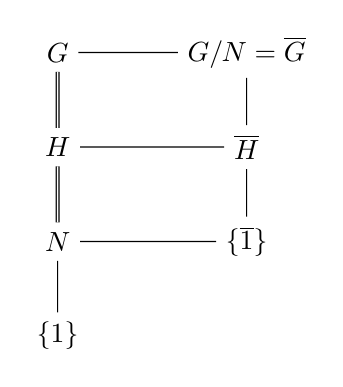
\begin{tikzpicture}[scale=1.2]
  % Nodes
  \node (G) at (-1,3) {$G$};
  \node (G/N) at (1,3) {$G/N=\overline{G}$};
  \node (H) at (-1,2) {$H$};
  \node (Hb) at (1,2) {$\overline{H}$};
  \node (N) at (-1,1) {$N$};
  \node (1b) at (1,1) {$\{\overline{1}\}$};
  \node (1) at (-1,0) {$\{1\}$};

  % Lineas nodos
  \draw[double] (G) -- (H);
  \draw[double] (H) -- (N);
  \draw (G) -- (G/N);
  \draw (G/N) -- (Hb);
  \draw (H) -- (Hb);
  \draw (Hb) -- (1b);
  \draw (N) -- (1b);
  \draw (N) -- (1);
\end{tikzpicture}
 
  \end{center}
\end{theorem}
\begin{proof} 
  Dado $\overline{H}\leq \overline{G}$, considere
  \begin{align*}
    H=\{g\in G: \pi(g)\in \overline{H}\}.
  \end{align*}
  Note que $N\normal G$, então $N\normal H$ e $\overline{H/N}$ por construção. 
\end{proof}
A correspondência preserva subgrupos normais, i,e. $\overline{H}\normal \overline{G}$ se, somente se, $H\normal G$.

Consequências do teorema do isomorfismo.
\begin{enumerate}
  \item Se $N\normal G$ e $H\leq G$, então
    \begin{itemize}
      \item $NH\leq G$.
      \item $N\normal NH$.
      \item $N\cap H\normal H$.
    \end{itemize}
    \begin{center}
      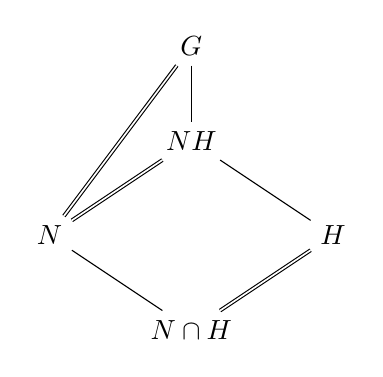
\begin{tikzpicture}[scale=1.2]
  % Nodos
  \node (G) at (0,3) {$G$};
  \node (NH) at (0,2) {$NH$};
  
  \node (N) at (-1.5,1) {$N$};
  \node (H) at (1.5,1) {$H$};
  
  \node (NcH) at (0,0) {$N\cap H$};
  
  % Aristas normales
  \draw (G) -- (NH);
  \draw (NH) -- (H);
  \draw (N) -- (NcH);
  
  % Aristas destacadas (dobles)
  \draw[double] (G) -- (N);
  \draw[double] (NH) -- (N);
  \draw[double] (H) -- (NcH);
\end{tikzpicture}

    \end{center}
    Temos $NH/N\cong H/N\cap H$, ja que se consideramos $\varphi:H\to NH/N$, definida por $\varphi(h)=Nnh=Nh$, logo $\varphi$ é sobrejetiva e $\ker\varphi=H\cap N$ (i,e. $\varphi$ é homomorfismo).
  \item $N\normal G$, $H\leq G$, com $N\leq H$. Se $H\normal G$, então $N/H\normal G/N$.
    \begin{align*}
      \frac{G/N}{H/N}\cong G/H.
    \end{align*}
    Basta considerar $\varphi:G/N\to G/H$ definido por $\varphi(Ng)=Hg$ e mostrar que $\varphi$ é homomorfismo sobrejetor tal que $\ker\varphi=H/N$. 
\end{enumerate}
Temos uma questão.
\begin{enumerate}
  \item Se todo subbgrupo próprio de $G$ é cíclico, é verdade que $G$ é cíclico? (Não, pode tomar como exemplo $S_3$).
  \item Se todo quociente próprio de $G$ é cíclico, então $G$ é cíclico? (Não, adivinhe o contraexemplo). 
\end{enumerate}
